\documentclass{article}
\usepackage[utf8]{inputenc}
\usepackage{graphicx}
\usepackage{amsmath}
\newcommand{\Tau}{\mathrm{T}}
\title{Dual Nature of Matter and Radiation}
\author{Amitesh Anand Pandey }
\date{October 2021}

\begin{document}

\maketitle
\section{Historic Advances}
\begin{itemize}
    \item \textbf{Wave Nature of Light}: James Clerk Maxwell and Heinrich Hertz's experiments on generation and detection of electromagnetic waves alongside Young's interference experiment using double slits established the wave nature of light.
    \item \textbf{Cathode Ray Experiment}: When two electrodes are kept in a discharge tube under 0.001 mm of Hg pressure, and an electric field is applied to the gas inside the discharge tube, the portion of glass opposite to the electrode develops color. This color has been attributed to a ray of particles. The cathode ray experiment suggested that a ray of particles appeared to be emitted from the cathode and deposited on the glass opposite to the cathode. \\  
    \begin{figure}[htp]
    \centering
    \includegraphics[width=5cm]{cr1.png}
    \caption{An image of the experiment}
    \label{fig:galaxy}
    \end{figure}
    \item \textbf{Discovery of the Electron}: By applying electric and magnetic fields mutually perpendicular to the cathode ray, J.J. Thompson deduced the particle's charge to mass ratio ($\frac{e}{m}$). In the same time period, it was found that a ray of particles very similar to the cathode rays are emitted when a metal is heated, or when light is shined on the metal. Thus, J.J. Thompson named these particles as electrons, and established their universality. 
    
    \newpage
    
    \item \textbf{Mass of an Electron}: As discussed above, J.J. Thompson deduced the charge by mass ratio of the electron. However, it was R.A. Millikan in his pioneering oil-drop experiment that found the specific value of the charge on an electron ($e = 1.6 \times 10^{-19} C$). This naturally also established the mass of an electron. 
\end{itemize}

\section{Emission of the Electron}
A metal has excess of electrons, some of which stay on the metal's surface. The electrons on the surface of a metal are bound to the metal by the attractive forces of the ions and protons inside the metal. A minimum amount of energy exists, which, when imparted to a surface electron of a specific metal, is sufficient for the electron to overcome the attractive forces and leave the metal. This minimum energy is called the \textbf{Work Function} ($\phi_{0}$) of the metal. \\ 

Various experiments have shown broadly three ways of imparting this minimum energy to metal surfaces to fuel the emission of electrons: 
\begin{enumerate}
    \item \textbf{Thermionic Emission}: By suitably heating the surface of a metal and imparting sufficient thermal energy. 
    \item \textbf{Field Emission}: By applying a very strong electric field ($10^{8} \ V m^{-1}$) to a metal surface.
    \item \textbf{Photoelectric Emission}: By illuminating the surface of a metal with a light of suitable frequency.
\end{enumerate}
\section{Photoelectric Effect}
\subsection{Hertz's Observations}
Hertz while conducting his experiments on the electromagnetic wave nature of light realised that the potential difference across a detector loop was enhanced when light fell on the metal's surface. Hertz hypothesised that the incident radiation imparted energy to the surface electrons which used that energy to overcome attractive forces and escape the metal with some kinetic energy. 

\subsection{Hallwachs' and Lenard's Observations}
 Lenard observed that when light illuminates the surface of an emitted plate in the vicinity of two electrodes, the emission of the particles results in the development of an external current in the circuit. This established that the beam of particles ejected out of the metal are charged particles.  
 Hallwachs later deduced that these charged particles carry a negative charge by illuminating the surface of a negatively charged zinc surface. He realised that the negatively charged zinc surface lost all of its excess charge after prolonged exposure to light. This concluded that the emitted ray carried electrons. 

\subsection{Experimental Arrangement}
In the arrangement for the study of the photoelectric effect, an incident light travels through a window and falls on the cathode plate. This results in the emission of electrons from the metallic cathode plate, and these electrons under the action of the electric field pre-developed by a potential difference between the cathode and anode plates, travel to the anode. This results in the development of a photo-current. 
    \begin{figure}[htp]
    \centering
    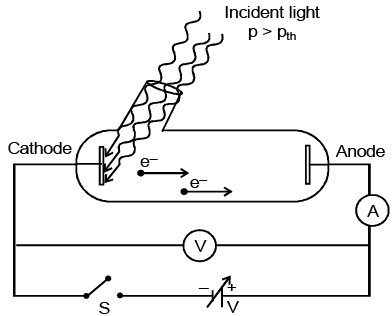
\includegraphics[width=5cm]{cr2.png}
    \caption{Arrangement of the experiment}
    \label{fig:galaxy}
    \end{figure}

This experimental setup can be used to determine the relation of photo-current with (a) intensity of radiation, (b) frequency of radiation, (c) the potential difference between the anode and cathode plates, and (d) the nature of the material of the cathode plate. \\ 

\textbf{Effect of intensity of incident light}: When the potential difference between the anode and cathode plates and the frequency of the incident light are both kept constant, and the intensity of the incident radiation is made to vary and each time, the the current is measured, we find that the intensity of the incident light varies linearly with the magnitude of the photo-current. 

\begin{figure}[htp]
    \centering
    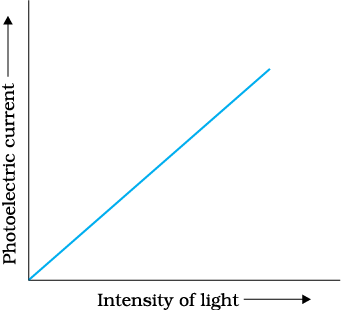
\includegraphics[width=4cm]{cr3.png}
    \caption{Photo-current vs Intensity of incident light}
    \label{fig:galaxy}
    \end{figure}
\newpage

\textbf{Effect of potential diff. of plates}: When the intensity of incident light ($I_{1}$) and also the frequency of incident light ($\nu$) are kept constant, while the potential on the anode plate is increased positively, it is observed that the photo-current increases up until the point that all electrons emitted by the cathode are received by the anode. At this point, the photo-current becomes constant and it is called the saturation current, or the saturation point. \\ 

On the other hand, if the potential on the anode is decreased until the point that it is no longer the anode, but carries negative potential, it is observed that at some sufficiently large negative potential on the ex-anode plate, the current completely stops flowing. This corresponds to the case when the negative potential on the ex-anode plate offers so much resistance to the emitted electrons from the ex-cathode plate, that no emitted electrons are able to make the journey and complete the current. This is also known as the stopping potential ($V_{0}$). \\

When we reach the point of the stopping potential on the ex-anode plate, it goes to show that the emitted electrons with the highest amount of kinetic energy ($K_{max}$) are still \emph{just} being resisted enough by the stopping potential ($V_{0}$) to complete their journey to the ex-anode plate. The mathematical formulation of this is:

\begin{equation}
    K_{max} = eV_{0}
\end{equation}
\\
Repeating  this experiment for incident radiations with fixed frequency but of different intensities ($I_{1}$, $I_{2}$, $I_{3}$) we find out that the the stopping potential is independent of the intensity, whereas the saturation current increases as $I$ increases. 


\begin{figure}[htp]
    \centering
    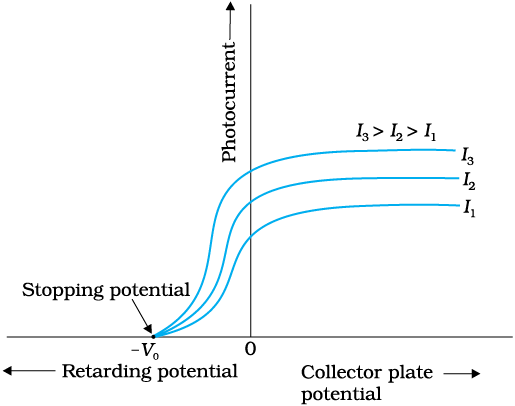
\includegraphics[width=6cm]{cr4.png}
    \caption{Photo-current vs Potential of Plates for different intensities of light}
    \label{fig:galaxy}
    \end{figure}

\newpage

\textbf{Effect of frequency of incident radiation on stopping potential}: When the intensity of the incident radiation is kept constant, and the frequency of the incident radiation is varied in the order $\nu_{3} > \nu_{2} > \nu_{1}$, it is observed that the different stopping potentials vary in the order $V_{03} > V_{02} > V_{01}$. This alongside the fact that $K_{max} = eV_{0}$ suggests that the maximum kinetic energy of emitted electrons increases as the frequency of incident light increases, whereas the saturation current stays constant.

\begin{figure}[htp]
    \centering
    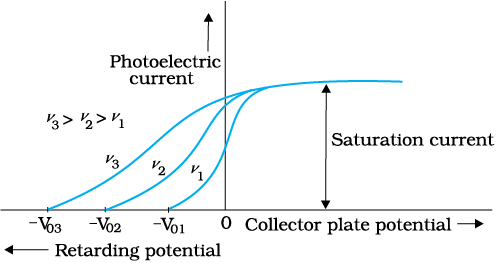
\includegraphics[width=6.5cm]{cr5.png}
    \caption{Photo-current vs Potential of Plates for different frequencies of light}
    \label{fig:galaxy}
    \end{figure}

When we plot the corresponding stopping potentials for incident lights of the same intensity but different frequencies, we observe that the stopping potential varies linearly with the frequency of incident light. However, the stopping potential is 0 until the frequency of incident light reaches a value of at least $\nu_{0}$. Repeating this experiment for two different metals concludes that this minimum sufficient value of frequency $\nu_{0}$ is dependent on the nature of the metal. 

\begin{figure}[htp]
    \centering
    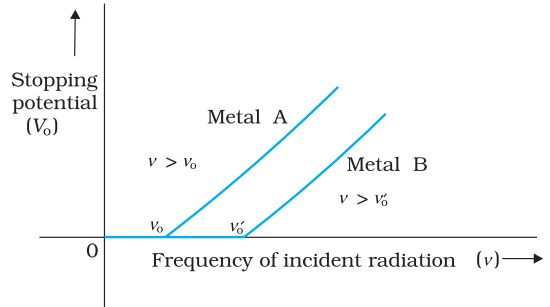
\includegraphics[width=7.5cm]{cr6.png}
    \caption{Stopping Potential vs Frequency of light for 2 metal plates}
    \label{fig:galaxy}
    \end{figure}

This minimum frequency which is required for the stopping potential to be non zero is called the threshold frequency. Regardless of the intensity of incident light, if its frequency is less than the threshold frequency, no photoelectric emission will take place. 

\newpage 

\subsection{Wave Nature of Light and Photoelectric Effect}

If we assume the wave nature of light, it is understood that an incident radiation of very high intensity will have a corresponding wave of very high amplitude. When this wave imparts energy to the electrons on the surface of a metal, regardless of the wave's frequency, the energy imparted should be so high that the electrons are emitted out. This however, contradicts our conclusion of the independence of the stopping potential from the intensity of the light. It also contradicts our result that suggests the existence of a threshold frequency at all. Moreover, it is observed that the emission of electron is instantaneous in the photoelectric effect, however, when a wave would hit the metallic surface, it would impart its energy somewhat uniformly to a very large pool of surface electrons, thereby making energy imparted per electron quite small. Calculations with the wave picture of light, and this small energy imparted per electron suggest that the photoelectric effect would take hours and days to complete. However, we know that it happens immediately. This goes to show the true incompatibility of the wave nature of light and the photoelectric effect.

\subsection{Einstein's Photoelectric Equation}
In Einstein's explanation of the photoelectric effect, instead of a wave picture, a particle picture of light is assumed. He posits that light travels in packets of energy called \emph{quanta} or photons. These photons have energies given by the equation:
\begin{equation}
    E = h \nu 
\end{equation}
where $h$ is the Planck's constant. Einstein continues to say that the energy imparted to a surface electron after contact with the photon is used partly to overcome the attractive forces and partly to emit the electron with a maximum kinetic energy. The mathematical formulation for this is: 
\begin{equation}
    h \nu = \phi_{0} + K_{max}
\end{equation}
The above equation manages to explain all of our inferences from the photoelectric experiment discussed in a prior section. If we assume $K_{max} = 0$ in the case when the electron barely manages to escape the metal, we get the relation:
\begin{equation}
    \nu_{0} = \frac{\phi_{0}}{h}
\end{equation}
This explains the existence of a threshold frequency. In this picture, the intensity of incident light manages the number of photons incident on the metal. If the number of photons incident on the metal are large, more electrons will be emitted, thereby increasing the photo-current. However, the intensity of the incident light does not affect the $K_{max}$ of a single electron or the stopping potential, which is in harmony with our results from the experiment. 

\newpage 

Using equations (1) and (3), we obtain the expression of the stopping potential for the photo-current as:

\begin{equation}
    V_{0} = (\frac{h}{e}) \nu - \frac{\phi_{0}}{e}
\end{equation}
This result accurately predicts our conclusion from the prior experiment that the stopping potential varies linearly with the frequency of incident light. Soon after Einstein published his model, R.A Millikan, the same man we attribute the discovery of the electron's charge and mass to, sought to disprove Einstein's model.  He performed a series of tests particularly on the metal sodium, and calculated the slope of the line ($\frac{h}{e}$). Using the value of the charge on an electron that he himself once derived, Millikan understood that the value of $h$ in this context was very close to the value of another constant that Max Planck had derived in an entirely different branch of physics. This suggested that the constant $h$, now called the Planck's constant was a fundamental physical quantity, and Millikan's experiments ended up adding more credibility to Einstein's model. 

\section{The Photon: A Particle?}
A.H. Compton about 1.5 decades after Einstein first produced his model, verified the existence of the particle-like nature of light through an experiment involving X-rays now called the Compton Electron Scattering Experiment. For his work in the Photoelectric Effect, Einstein was awarded the Nobel Prize in physics in 1921, and for his work in the discovery of the physical properties of the electron as well as the Photoelectric Effect, Millikan was awarded the Nobel Prize in physics in 1923. \\ \\
Some properties (energy, velocity, momentum respectively) of the photon are:

\begin{equation}
    E_{photon} = h \nu = \frac{hc}{\lambda}
\end{equation}
\begin{equation}
    v_{photon} = c \text{ (speed of light)}
\end{equation}
\begin{equation}
    p_{photon} = h \frac{\nu}{c} = \frac{h}{\lambda}
\end{equation}
\section{Wave Nature of Matter}
In 1924, Louis Victor de Broglie questioned: If EM waves can behave as particles in some cases, cannot the particles also demonstrate wave-like nature in some cases? de Broglie argued that the nature is symmetrical and matter should preserve the symmetry observed in waves by showing wave-like nature. de Broglie hypothesised that the wavelength ($\lambda$) of the wave of a particle is given by:
\begin{equation}
    \lambda = \frac{h}{p} = \frac{h}{mv}
\end{equation}
Using de Broglie's relation, we can find the expected value of the de Broglie wavelength of an electron accelerated by a potential difference $V$ as follows:

\begin{equation}
    K.E = eV 
\end{equation}
\begin{equation}
    K.E = \frac{p^{2}}{2m}
\end{equation}
\begin{equation}
    p = \sqrt{2meV}
\end{equation}
\begin{equation}
    \lambda = \frac{h}{p} = \frac{h}{\sqrt{2meV}}
\end{equation}
Substituting the value for the mass of an electron ($m$), the Planck's constant ($h$), and the charge on an electron ($e$), we obtain the relation:
\begin{equation}
    \lambda = \frac{1.227}{\sqrt{V}}
\end{equation}
\section{Davisson-Germer Experiment}
The result of the Davisson-Germer experiment was the observation of a peak value in the intensity of the scattered electron wave at 54V of supply voltage. This peak value occurred due to constructive interference of scattered electrons. The calculated wavelength from the electron diffraction measurements in the Davisson-Germer experiment was equal to: $0.165$ nm.  \\ \\

If we use equation 14. derived from the de Broglie relation to calculate the wavelength of an electron wave from an electron accelerated by a potential difference of 54V, we observe:
\begin{equation}
    \lambda = \frac{1.227}{\sqrt{54}} = 0.167 \ \text{nm}
\end{equation}
This value is shockingly close to the value observed by Davisson-Germer at 54V. This, along with C.G. Thompson's experiments on the diffraction of electrons in a crystal proved de Broglie's hypothesis and won him the Nobel prize alongside Davisson and C.G. Thompson. 
\end{document}
